\documentclass[svgnames]{article}    

\usepackage{graphicx}                 

% -- math                               
\usepackage{amssymb}
\usepackage{amsmath}
\usepackage{esint}
\usepackage{geometry}

% -- noindent
\setlength\parindent{0pt}

% -- images

% -- tikz
\usepackage{pgfplots}
\pgfplotsset{compat=1.15}
\usepackage{comment}
\usetikzlibrary{arrows}
\usepackage[most]{tcolorbox}

\newtcolorbox{mybox}{
    enhanced,
    boxrule=0pt,frame hidden,
    colback=green!10!white,
    sharp corners
}

% -- figures


% -- figures
\usepackage{float}
\usepackage{caption}
\usepackage{lipsum}

% -- start 
\title{Fitting}
\author{Deval Deliwala}
%\date{}                              

\begin{document}
\maketitle
%\tableofcontents 


Lew, in his thesis, uses three compound derivative Lorentzians with the following form, 

\[
    \Delta I ( B_0 ) = \Delta I_{CP} \left( \frac{\Delta B^2}{\Delta B^2 +
    B_0^2} \right),  
\] \vspace{3px}

to model his 4H-SiC EDMR spectra. We will be attempting a similar
compound-Lorentzian fit on our 2Gauss, 3Volt, 200MHz EDMR spectra. But first, we
will derive the fit functional form from first principle spin mechanics. \\

This derivation mimics the one presented in Lew Chapter 3, but slightly
modified. 

\section{Single-spin dynamics}

\subsection{Magnetic Moment and Torque}

For an electron of charge $q = -e$ and mass $m$, the magnetic moment $\vec{\mu}$ 

\[
    \vec{\mu} = -g_e \mu_B \frac{\vec{S}}{\hbar}, \qquad \mu_B =
    \frac{e\hbar}{2m}. 
\] \vspace{3px}

The torque on the moment in a magnetic field  $\vec{B}$ is 

\[
\vec{\tau} = \frac{d \vec{S}}{dt} = \vec{\mu} \times \vec{B}.
\] \vspace{3px}

Inserting $\vec{\mu}$ and defining the gyromagnetic ratio $\gamma = g_e \mu_B /
\hbar$ : 

\[
\frac{d \vec{S}}{d t} = -\gamma \vec{S} \times \vec{B}. 
\] 

\subsection{Larmor Precession} 

For a static field $\vec{B}_0 = B_0 \hat{z}$, the solution is a uniform
precession about $\hat{z}$: 

\[
\vec{S}(t) = \begin{pmatrix}
    S_\perp \cos(\omega_0 t + \phi) \\ S_\perp \sin(\omega_0 t + \phi) \\ S_z(0)
\end{pmatrix} , \quad \omega_0 = |\gamma| B_0.
\] \vspace{3px}

The Larmor condition is when $\omega = \omega_0$; when the external drive
matches the mechanical eigen-frequency, energy can be absorbed resonantly. 

\section{The Bloch Equations} 

\subsection{Classical Magnetisation}

Let the bulk magnetisation $\vec{M} = \sum_i \langle \mu_i \rangle / V$.
Averaging the single-spin torque and adding the relaxation terms $T_1$ and $T_2$
gives 

\[
    \frac{d \vec{M}}{d t} = \gamma \vec{M} \times \vec{B} - \frac{M_x \hat{x} +
    M_y \hat{y}}{T_2} - \frac{(M_z - M_0)\hat{z}}{T_1}. 
\] \vspace{3px}

$T_1$ drives $M_z \rightarrow M_0$ (longitudinal relaxation). $T_2$ damps
transverse coherence. Our EDMR spectra is taken while sweeping a static field
$B \hat{z}$ through resonance while applying a continuous transverse RF field of
fixed angular frequency $\omega$: 

\[
\vec{B}(t) = B \hat{z} + 2B_1 \cos(\omega t) \hat{x}. 
\] \vspace{3px}

where the factor of 2 is for simplifying algebra later on with the rotating-wave
approximation. $B_1$ is the rms amplitude. 

\section{Rotating Frame Transformation}

Define a frame that rotates \textit{about} $\hat{z}$ at the drive frequency
$\omega$. Let $\vec{M}_\text{lab} $ be the lab vector and $\vec{M}$ the
rotating-frame vector. Then, 

\[
    \frac{d \vec{M}_\text{lab} }{d t} \Big|_\text{lab} = \frac{d \vec{M}}{dt}
    \Big|_\text{rot} + \omega \hat{z} \times \vec{M}.
\] \vspace{3px}

Insert this into the Bloch equations defined above to yield 

\[
\frac{d \vec{M}}{d t} = \gamma \vec{M} \times \vec{B}_\text{eff} - \frac{M_x
\hat{x} + M_y \hat{y}}{T_2} - \frac{(M_z - M_0) \hat{z}}{T_1}, 
\] \vspace{3px}

with an effective field of 

\begin{align} \label{Beff}
    \vec{B}_\text{eff}  = (B - \omega / \gamma) \hat{z} + B_1 \hat{x}. 
\end{align}

The effective field was derived by the \textit{rotating-wave approximation}: 

\[
    2B_1 \cos \omega t \hat{x} = B_1(e^{+i\omega t} + e^{-i\omega t} ) \hat{x}. 
\] \vspace{3px} 

In the frame co-rotating at $+\omega$, the $e^{+i\omega t}$ piece is static,
while the $e^{-i\omega t}$ term oscillates at $2\omega$. Provided $\omega \gg
1/T_2$, we drop the latter. What remains is the static $B_1 \hat{x}$ present in
$\vec{B}_\text{eff}$. 

Now in steady state (not pulsed) EDMR, we set $d\vec{M} / dt = 0$ and let
$\Delta \omega = \omega - \gamma B.$ Therefore, with the unknowns $M_x, M_y,
M_z$, we get a $3 \times 3$ linear system: 

\[
\begin{cases}
    0 = \gamma \left( M_y B_{\text{eff}, z} - M_z B_1 \right) - \dfrac{M_x}{T_2}, \\ 
    0 = \gamma \left( M_z B_1 - M_x B_{\text{eff}, z} \right) - \dfrac{M_y}{T_2}, \\ 
    0 = \gamma \left( M_x B_1 - M_y B_1 \right) - \dfrac{M_z - M_0}{T_1}.
\end{cases}
\] \vspace{3px}

From Equation \ref{Beff}, we see $B_\text{eff, z} = -\Delta \omega / \gamma$.
Therefore, the first two equations couple only through $B_1$ and $\Delta
\omega$. Solving yields the solutions 

\begin{align}
    M_x &= \frac{\gamma B_1 T_2 M_0}{1 + (\Delta \omega T_2)^2 + \gamma^2 B_1^2
  T_1T_2}, \\ 
        M_y &= \frac{\gamma B_1 T_2 (\Delta \omega T_2) M_0}{1 + (\Delta \omega
        T_2)^2 + \gamma^2 B_1^2 T_1T_2}, \\ 
            M_z &= \frac{M_0}{1 + (\gamma B_1)^2 T_1T_2 + (\Delta \omega
            T_2)^2}.
\end{align} \vspace{3px}

\section{Lorentzian Line Shape}

Now is where things get a bit hand-wavy. The derivation from now on isn't fully
firm but is a good heuristic for fitting. 

Again from Equation \ref{Beff}, we have 

\[
    \vec{B}_\text{eff} = B_z \hat{z} + B_1 \hat{x}, \qquad B_z \equiv
    \frac{\Delta \omega}{\gamma}, \quad \Delta \omega = \omega - \gamma B.
\] \vspace{3px}

Inserting this into the Bloch equations at steady state ($d M_z / dt = 0$) and
linearising the equations in  $B_1$, we get 

\begin{align} \label{mdot}
    \dot{M_x} &= -\Delta \omega M_y - \frac{M_x}{T_2} + 0 \cdot B_1, \\ 
    \dot{M_y} &= +\Delta \omega M_x - \frac{M_y}{T_2} + \gamma M_0B_1. 
\end{align}\vspace{3px}


We now solve Equation \ref{mdot} in the frequency domain. Defining the complex
transverse magnetization 

\[
    M_+(t) \equiv M_x(t) + iM_y(t), \qquad B_+(t) \equiv 2B_1e^{-i\omega t}.
\] \vspace{3px}

Taking the fourier transform and solving yields 

\begin{align} \label{comptrans}
M_+(\omega) = \gamma M_0 B_1 \frac{1}{1/T_2 - i\Delta \omega}. 
\end{align} \vspace{3px}

Now Equation \ref{comptrans} has the form of 

\[
M_+(\omega) = \chi_0 \frac{1}{\chi(\omega)}B_1,
\] \vspace{3px}


so the \textit{complex transverse susceptibility} is 

\[
\chi(\omega) = \frac{\chi_0 T_2}{1 - i\Delta \omega T_2} 
\] \vspace{3px}

Separating this into its real and imaginary parts yields 

\begin{align} \label{reim}
    \chi'(\omega) = \Re\{\chi(\omega)\} &= \frac{\chi_0 T_2}{1 + (\Delta \omega T_2)^2} \\ 
    \chi''(\omega) = \Im\{\chi(\omega)\} &= \frac{\chi_0 T_2^2 \Delta \omega}{1+(\Delta \omega
    T_2)^2}
\end{align}\vspace{3px}

Turns out, the energy a spin system absorbs is proportional to the imaginary
$\Im$
part. Therefore, any measurable change in EDMR current -- a result of energy
absorption -- is proportional to $\chi''(\omega) $. Therefore, we have 

\[
\Delta I(B) \propto \frac{\Delta \omega T_2}{1 + (\Delta \omega T_2)^2} 
\] \vspace{3px}

Now, letting the half-width at half-maximum 

\[
\Gamma \equiv \frac{1}{|\gamma| T_2}
\] \vspace{3px}

Inserting this into $\chi''$, and switching to the field axis $\Delta \omega =
\gamma(B - B_\text{res})$, we get 

\begin{align} \label{current}
\Delta I(B) \propto \frac{\Gamma^2}{\Gamma^2 + (B - B_\text{res})^2}. 
\end{align} \vspace{3px}

which is an exact Lorentzian. 

\section{Lock-in Amplifier}

Here, I believe in our EDMR setup, to reduce noise and distinguish the
spin-dependent current changes from the background, we add a small
\textit{sine}-wave to the static magnetic field. Specifically, there is a small
$\delta B$ modulation in addition to the static applied $B_0$. The instantaneous
field experienced by the spins is then 

\[
B(t) = B_0 + \delta B \cos \Omega t \qquad (\delta B \ll B_0).
\] \vspace{3px}


We expand the current 

\[
    I(B(t)) \approx I(B_0) + \frac{\partial I}{\partial B} \Big|_{B_0} \delta B
    \cos \Omega t + \mathcal{O}(\delta B^2)
\] \vspace{3px}


Since EDMR uses a lock-in amplifier, we define the lock-in amplifier's
\textit{demodulted} output, the actual observed spectra as 

\begin{align} \label{lockin}
    S(B_0) = \frac{2}{T_\text{avg} }\int_{t_0}^{t_0 + T_\text{avg} } I(B_0 +
    \delta B \cos \Omega t)\cos\Omega t  \, dt
\end{align}\vspace{3px}

Therefore, if we expand to first-order, we get 

\[
I(B_0 + \delta B \cos\Omega t) \cdot \cos \Omega t \approx I(B_0)
\cos\Omega t + \frac{\partial I}{\partial B}
\Big|_{B_0} \delta B \cos^2 \Omega t + \mathcal{O}(\delta B^2)
\] \vspace{3px}

We can solve the integral by just averaging, 

\begin{align*}
    \langle I(B_0) \cos \Omega t \rangle &= I(B_0) \langle \cos \Omega t\rangle
    = 0 \\ 
    \langle \cos^2 \Omega t \rangle &= \frac{1}{2}
\end{align*}


Hence, 

\begin{align}\label{obs}
    S(B_0) = \frac{2}{T_\text{avg}} \int \left[ I(B_0) + I'(B_0)\delta B
    \cos\Omega t \right] \cos \Omega t dt = \frac{\delta B}{2} \frac{\partial I}{\partial B}\Big|_{B_0}
\end{align} \vspace{3px}

The lock-in outputs a current proportional to the \textbf{first derivative} of
the underlying $I(B)$. This is what is being observed in the EDMR spectra. 


\section{Markov Chain Monte Carlo (MCMC)}

\begin{figure}[H]
  \centering
    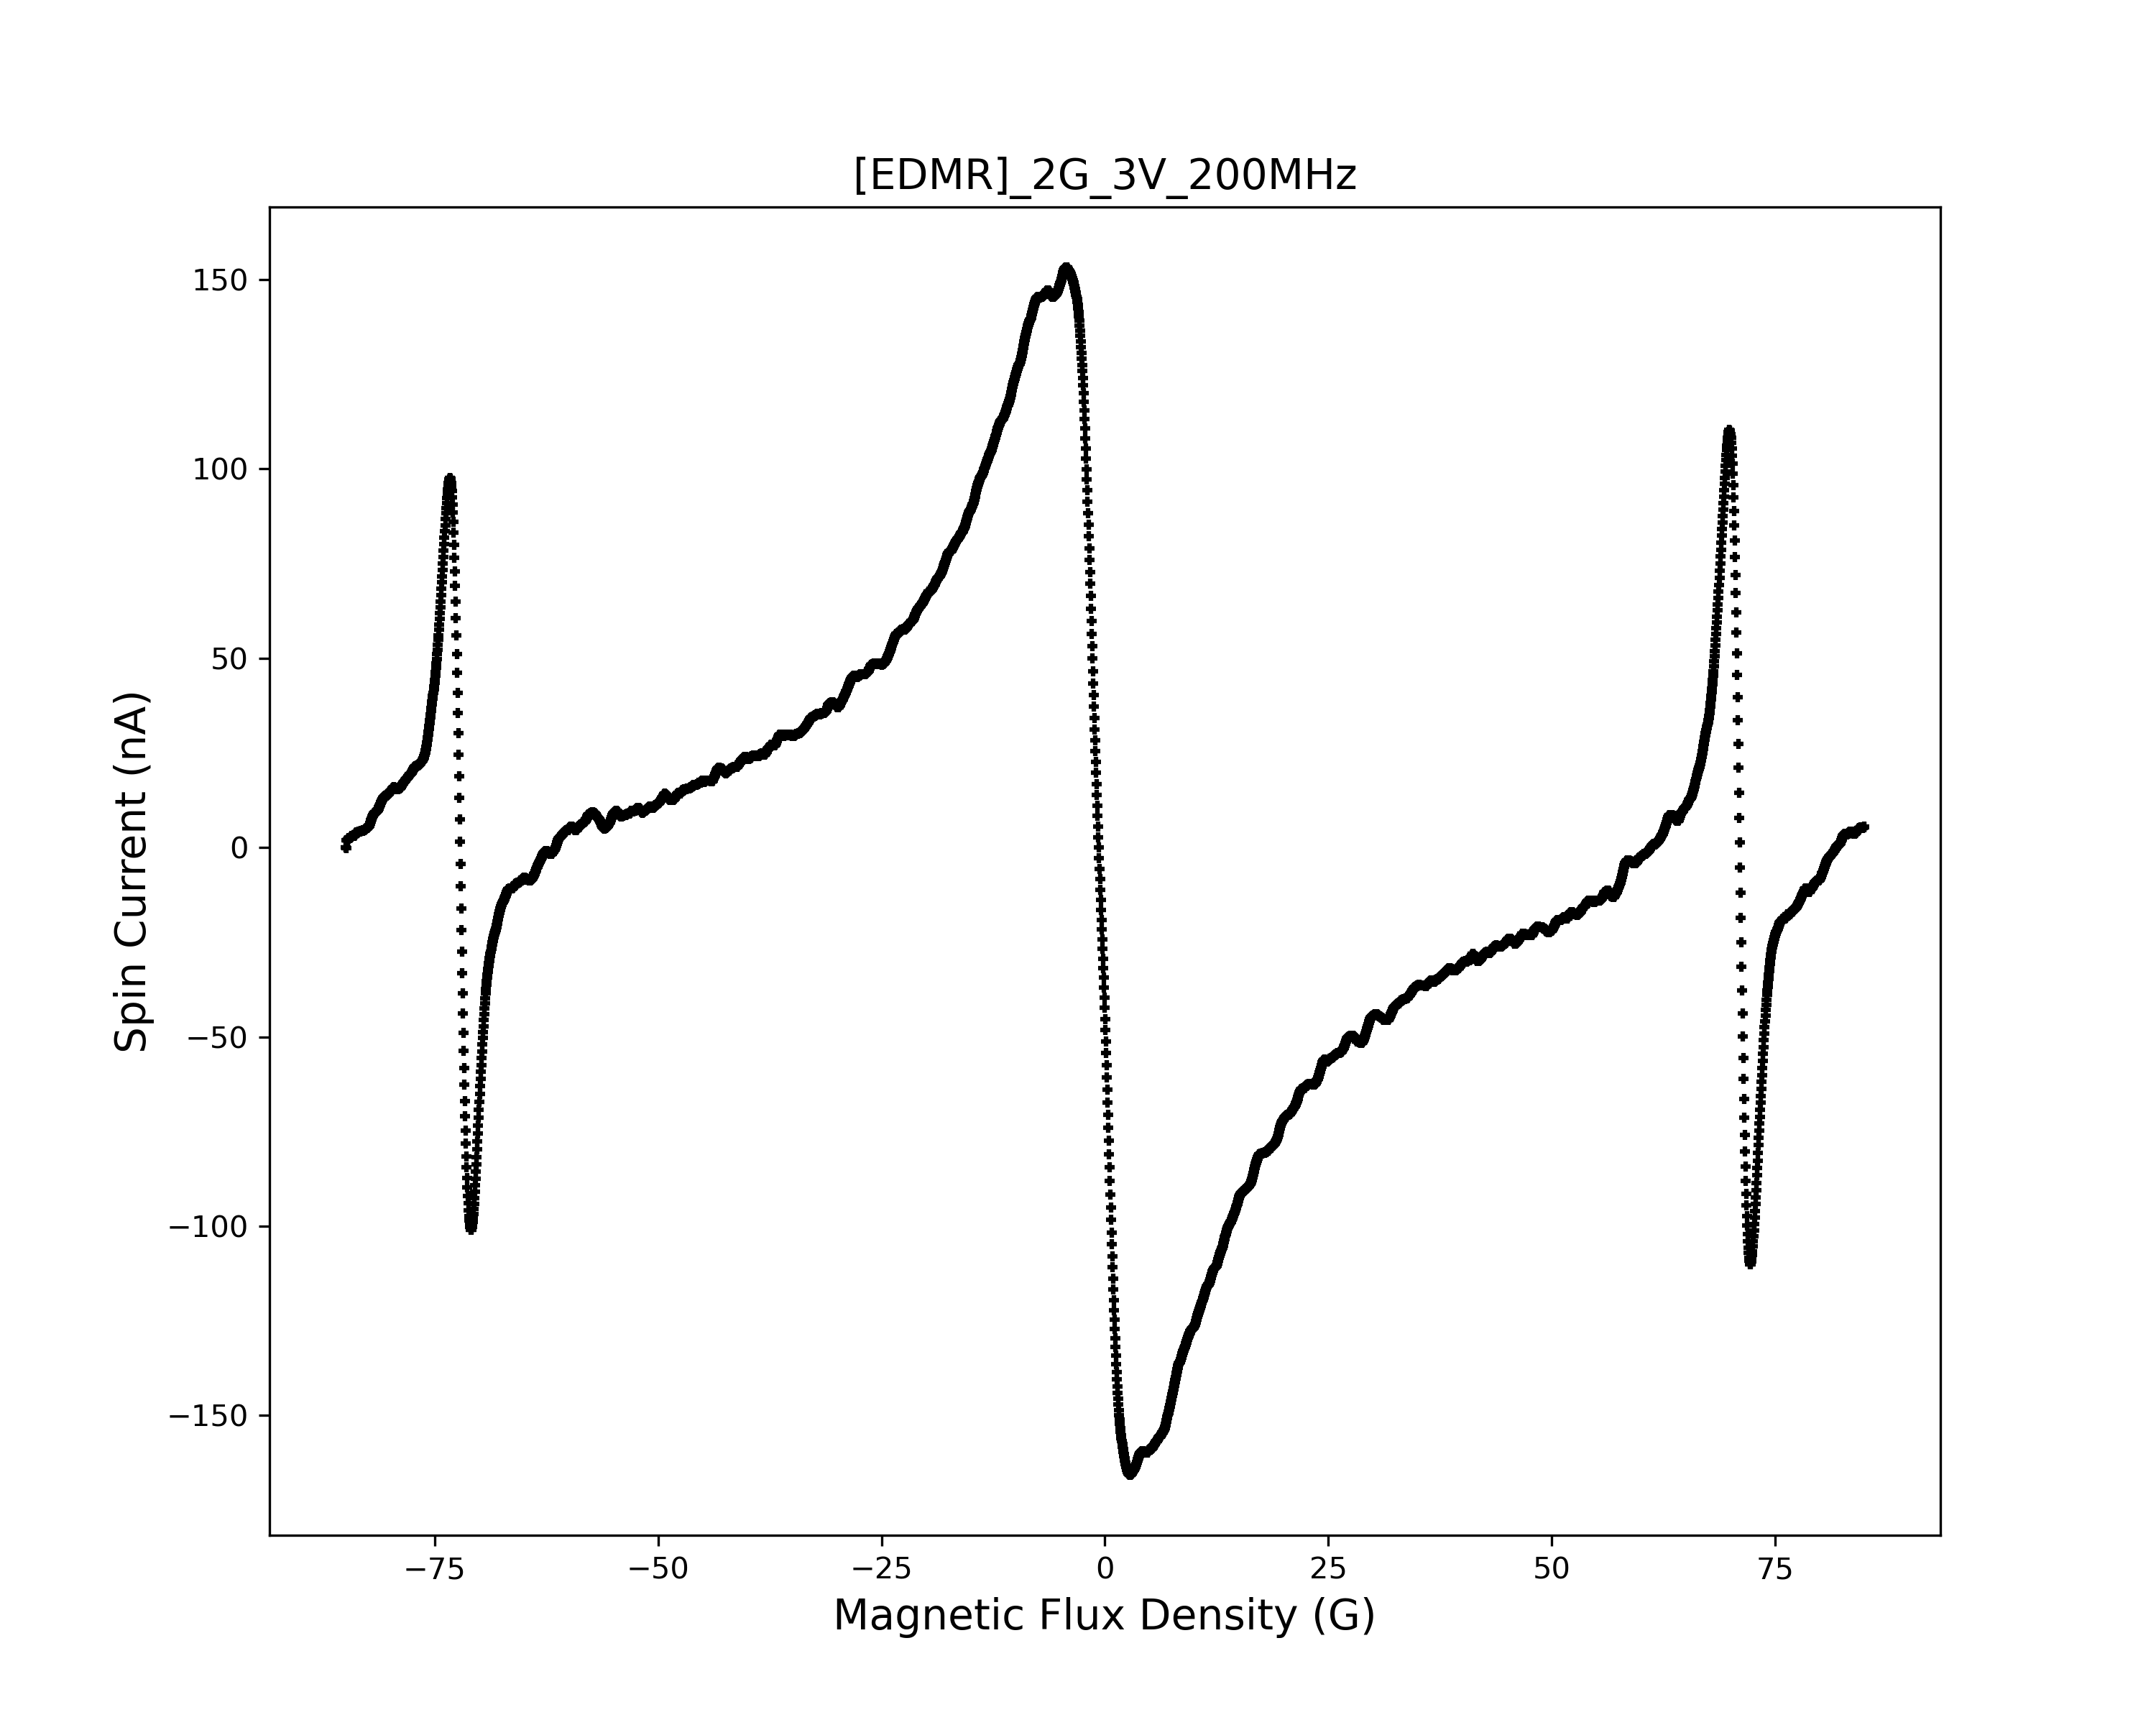
\includegraphics[width = \linewidth]{spectra.png} 
    \caption{EDMR spectra at 2G, 3V, and 200MHz. It can be modeled via three
    compound-lorentzian derivatives.}
\end{figure}



From Equation \ref{current}, we have 

\[
\Delta I (B) = C \frac{\Gamma^2}{\Gamma^2 + (B-B_\text{res} )^2}, \qquad \Gamma
= \frac{1}{|\gamma|T_2}
\] \vspace{3px}

We differentiate the above equation and insert it into Equation \ref{obs}: 

\[
S(B) = -2A \frac{B}{(B^2 + \Gamma^2)^2}, \qquad A \equiv \frac{\delta
B}{2}C\Gamma^2.
\] \vspace{3px}

This is the first derivative of a centered Lorentzian. Empirically, the EDMR
spectra constitutes three independent processes (hyperfine, zero-field, possibly
relaxation ?) Therefore the compound model follows 

\[
S_\text{model}(B; \; \theta) = S_0 - 2B \sum_{k=1}^{3} \frac{A_k}{(B^2 +
\Gamma_k^2)^2},  
\] \vspace{3px}

with parameter vector 

\[
\theta = (S_0, A_1, A_2, A_3, \Gamma_1, \Gamma_2, \Gamma_3, \sigma). 
\] \vspace{3px}

where $S_0$ is the baseline offset and $\sigma$ is the stddev of the Gaussian
noise. There exists an implicit $T_2$ within each fitted $\Gamma_k$. $T_1$ does
not appear. 

\subsection{Likelihood}

For measured pairs $\{B_i, S_i\}_{i=1}^N$, where $N$ is the number of random
walkers and independent Gaussian noise:

\[
    \mathcal{L}(\theta) = \prod_{i=1}^N \frac{1}{\sqrt{2\pi}\sigma} \text{exp}
    \left[ -\frac{(S_i - S_\text{model}(B_i; \; \theta))^2 }{2\sigma^2}\right]
\] \vspace{3px}

Therefore, 

\[
    \ln \mathcal{L} = -N \ln \sigma - \frac{1}{2\sigma^2} \sum_{i=1}^{N} \left[
    S_i - S_\text{model}(B_i; \; \theta)\right]^2 - \frac{N}{2}\ln(2\pi). 
\] \vspace{3px}

\subsection{Priors}

 We adopt weakly informative priors without any biases: 

\begin{align*}
    S_0 &\quad \sim \mathcal{U}\left[ \text{min} S_i,, \text{max} S_i\right] \\ 
    A_k &\quad \sim \mathcal{N}(0, 200\text{nA}^2 ) \\ 
    \Gamma_k &\quad \sim \log\mathcal{U}\left[0.05, 100\right] \text{G} \\ 
    \sigma &\quad \sim \text{Half-Cauchy} 
\end{align*}

The final posterior is then 

\[
    \ln P(\theta | \text{ data} ) = \ln \mathcal{L}(\theta) + \sum_{\xi \in
    \theta}^{} \ln p(\xi).  
\] \vspace{3px}

\section{Future work}

This derivation is focused on the $\pm 50$G region of the spectra and does not
include the resonance peaks beyond  $\pm 70$G. To get a full description of an
infinitely-long spectra in gauss-space, we could use a ``gauss-series" similar
to a time-series and do a compound fourier lorentzian-derivative fit that
repeats at every resonance condition dependending on the material. This would be
very interesting and doable. But for now, I'll work on coding this main
zero-field fit and getting some results.\\ 



https://journals.aps.org/prb/abstract/10.1103/PhysRevB.76.054409 \\
https://journals.aps.org/prl/abstract/10.1103/PhysRevLett.130.266703 \\ 
All-electrical Quantum Sensing with Silicon Carbide Devices -- Christopher
Tao-Kuan Lew \\
https://en.wikipedia.org/wiki/Bloch\_equations (wikipedia I know) \\ 








\end{document}
